\section{FEM}

\subsection{FEM Ergebnisse}
  \label{FEM Ergebnisse}

  \subsubsection{FEM-Ergebnis - Lastfall 1.1 Vertikale Beschleunigung}
  \begin{table}[H]
  \centering
  \begin{tabular}{lcccccc}
  Grösse	&	Einheit	&	x	&	y	&	z	&	Total	&	Berechnet	\\	\hline
  \multicolumn{5}{l}{\textbf{Lagerreaktionen}}									&		&		\\	\thickhline
  Deichsel	&	N	&	0	&	3193	&	0	&	3193	&	-1028	(y) \\
  Chassis Links	&	N	&	0	&	35171	&	6733	&	35810	&	37300 (y)	\\
  Chassis Rechts	&	N	&	0	&	35171	&	-6733	&	35810	&	37300 (y)	\\	\hline	\\
  \multicolumn{5}{l}{\textbf{Chassis}}									&		&		\\	\thickhline
  Axialkraft	&	N	&		&		&		&	-50730	&	-44518	\\
  Querkraft	&	N	&		&		&		&	17003	&	19079	\footnotemark \\
  Biegemoment	&	kNmm	&		&		&		&	16980	&		\\	\hline	\\
  \multicolumn{5}{l}{\textbf{Dach}}									&		&		\\	\thickhline
  Axialkraft	&	N	&		&		&		&	2879	&	14840	\\
  Querkraft	&	N	&		&		&		&	108	&		\\
  Biegemoment	&	kNmm	&		&		&		&	42	&		\\	\hline	\\
  \multicolumn{5}{l}{\textbf{Träger A und B}}													\\	\thickhline
  Axialkraft	&	N	&		&		&		&	-10904	&		\\
  Querkraft	&	N	&		&		&		&	1293	&		\\
  Biegemoment	&	kNmm	&		&		&		&	327	&		\\	\hline	\\
  \multicolumn{5}{l}{\textbf{Kontaktreaktion: Chassis - Träger A und B}}									&		&		\\	\thickhline
   Axialkraft A	&	N	&	-620	&	12931	&	-218	&	12948	&		\\
  Biegemoment A	&	kNmm	&	-4602	&	-179	&	341	&	4618	&		\\
  Axialkraft B	&	N	&	2464	&	15784	&	713	&	15991	&		\\
  Biegemoment B	&	kNmm	&	-5610	&	851	&	-346	&	5685	&		\\	\hline	\\
  \multicolumn{5}{l}{\textbf{Kontaktreaktion: Chassis - Boden}}									&		&		\\	\thickhline
  Normalkraft (Zug)	&	N	&		&		&		&	883	&		\\
  Schubkraft (xz-Ebene)	&	N	&		&		&		&	9933	&		\\	\hline
  \end{tabular}
  \caption{Resultate der FEM-Simulation des Lastafalles der vertikalen Beschleunigung}
  \label{tab:FEM 1.1}
  \end{table}
  \footnotetext[2]{Unter der Annahme, dass nur das Chassis Querkräfte aufnimmt. Die Kraft von 19 kN ergibt sich aus der Halbierung der globalen Querkraft aus der Berechnung im Kapitel \ref{1.1 Vertikale Beschleunigung}.}

  \subsubsection{FEM-Ergebnis - Lastfall 1.3 Longitudinale Beschleunigung negativ}
  \begin{table}[H]
  \centering
  \begin{tabular}{lcccccc}
  Grösse	&	Einheit	&	x	&	y	&	z	&	Total	&	Berechnet	\\	\hline
  \multicolumn{5}{l}{\textbf{Lagerreaktionen}}									&		&		\\	\thickhline
  Deichsel	&	N	&	-20611	&	-3050	&	0	&	20835	&	206000 (x)	\\
  Chassis Links	&	N	&	0	&	1525	&	515	&	1610	&		\\
  Chassis Rechts	&	N	&	0	&	1525	&	-515	&	1610	&		\\	\hline	\\
  \multicolumn{5}{l}{\textbf{Chassis}}									&		&		\\	\thickhline
  Axialkraft	&	N	&		&		&		&	6080	&		\\
  Querkraft	&	N	&		&		&		&	1319	&		\\
  Biegemoment	&	kNmm	&		&		&		&	2601	&		\\	\hline	\\
  \multicolumn{5}{l}{\textbf{Dach}}									&		&		\\	\thickhline
  Axialkraft	&	N	&		&		&		&	553	&		\\
  Querkraft	&	N	&		&		&		&	8	&		\\
  Biegemoment	&	kNmm	&		&		&		&	2	&		\\	\hline	\\
  \multicolumn{5}{l}{\textbf{Träger A und B}}													\\	\thickhline
  Axialkraft	&	N	&		&		&		&	-1562	&		\\
  Querkraft	&	N	&		&		&		&	56	&		\\
  Biegemoment	&	kNmm	&		&		&		&	17	&		\\	\hline	\\
  \multicolumn{5}{l}{\textbf{Kontaktreaktion: Chassis - Träger A und B}}									&		&		\\	\thickhline
   Axialkraft A	&	N	&	-56	&	2084	&	325	&	2110	&		\\
  Biegemoment A	&	kNmm	&	-734	&	-19	&	2	&	734	&		\\
  Axialkraft B	&	N	&	98	&	667	&	80	&	679	&		\\
  Biegemoment B	&	kNmm	&	-236	&	34	&	-14	&	238	&		\\	\hline	\\
  \multicolumn{5}{l}{\textbf{Kontaktreaktion: Chassis - Boden}}									&		&		\\	\thickhline
  Normalkraft (Zug)	&	N	&		&		&		&	35	&		\\
  Schubkraft (xz-Ebene)	&	N	&		&		&		&	1733	&		\\	\hline
  \end{tabular}
  \caption{Resultate der FEM-Simulation des Lastafalles der longitudinalen Beschleunigung}
  \label{tab:FEM 1.3}
  \end{table}


  \subsubsection{FEM-Ergebnis - Lastfall 1.4 laterale Beschleunigung}
  \begin{table}[H]
  \centering
  \begin{tabular}{lcccccc}
  Grösse	&	Einheit	&	x	&	y	&	z	&	Total	&	Berechnet	\\	\hline
  \multicolumn{5}{l}{\textbf{Lagerreaktionen}}									&		&		\\	\thickhline
  Deichsel	&	N	&	0	&	0	&	1023	&	1023	&	-330 (z)	\\
  Chassis Links	&	N	&	0	&	-15008	&	11290	&	18780	&	11900 (z)	\\
  Chassis Rechts	&	N	&	0	&	15008	&	11242	&	18752	&	11900 (z)	\\	\hline	\\
  \multicolumn{5}{l}{\textbf{Chassis}}									&		&		\\	\thickhline
  Axialkraft	&	N	&		&		&		&	-31674	&	-11480	\\
  Querkraft	&	N	&		&		&		&	7163	&	6100	\footnotemark \\
  Biegemoment	&	kNmm	&		&		&		&	6658	&		\\	\hline	\\
  \multicolumn{5}{l}{\textbf{Dach}}									&		&		\\	\thickhline
  Axialkraft	&	N	&		&		&		&	-2560	&	-964	\\
  Querkraft	&	N	&		&		&		&	24	&		\\
  Biegemoment	&	kNmm	&		&		&		&	13	&		\\	\hline	\\
  \multicolumn{5}{l}{\textbf{Träger A und B}}													\\	\thickhline
  Axialkraft	&	N	&		&		&		&	2684	&		\\
  Querkraft	&	N	&		&		&		&	1067	&	470	\\
  Biegemoment	&	kNmm	&		&		&		&	627	&	470	\\	\hline	\\
  \multicolumn{5}{l}{\textbf{Kontaktreaktion: Chassis - Träger A und B}}									&		&		\\	\thickhline
   Axialkraft A	&	N	&	237	&	-3577	&	1729	&	3979	&		\\
  Biegemoment A	&	kNmm	&	1924	&	71	&	-102	&	1928	&		\\
  Axialkraft B	&	N	&	-733	&	-4221	&	1679	&	4602	&		\\
  Biegemoment B	&	kNmm	&	2097	&	-251	&	95	&	2114	&		\\	\hline	\\
  \multicolumn{5}{l}{\textbf{Kontaktreaktion: Chassis - Boden}}									&		&		\\	\thickhline
  Normalkraft (Zug)	&	N	&		&		&		&	1942	&		\\
  Schubkraft (xz-Ebene)	&	N	&		&		&		&	10972	&		\\	\hline
  \end{tabular}
  \caption{Resultate der FEM-Simulation des Lastafalles der lateralen Beschleunigung}
  \label{tab:FEM 1.4}
  \end{table}
  \footnotetext[3]{Unter der Annahme, dass nur das Chassis Querkräfte aufnimmt. Die Kraft von 6.1 kN ergibt sich aus der Halbierung der globalen Querkraft aus der Berechnung im Kapitel \ref{1.4 Laterale Beschleunigung}.}


  \subsubsection{FEM-Ergebnis - Lastfall 1.5 Rotatorische Beschleunigung}
  \begin{table}[H]
  \centering
  \begin{tabular}{lcccccc}
  Grösse	&	Einheit	&	x	&	y	&	z	&	Total	&	Berechnet	\\	\hline
  \multicolumn{5}{l}{\textbf{Lagerreaktionen}}									&		&		\\	\thickhline
  Deichsel	&	N	&	0	&	0	&	804	&	804	&		\\
  Chassis Links	&	N	&	0	&	-23097	&	10913	&	25546	&	-27000 (y)	\footnotemark \\
  Chassis Rechts	&	N	&	0	&	23097	&	10844	&	25516	&	27000 (y)	\\	\hline	\\
  \multicolumn{5}{l}{\textbf{Chassis}}									&		&		\\	\thickhline
  Axialkraft	&	N	&		&		&		&	-44164	&		\\
  Querkraft	&	N	&		&		&		&	10927	&		\\
  Biegemoment	&	kNmm	&		&		&		&	10218	&		\\	\hline	\\
  \multicolumn{5}{l}{\textbf{Dach}}									&		&		\\	\thickhline
  Axialkraft	&	N	&		&		&		&	-3625	&		\\
  Querkraft	&	N	&		&		&		&	32	&		\\
  Biegemoment	&	kNmm	&		&		&		&	19	&		\\	\hline	\\
  \multicolumn{5}{l}{\textbf{Träger A und B}}													\\	\thickhline
  Axialkraft	&	N	&		&		&		&	-4119	&		\\
  Querkraft	&	N	&		&		&		&	1311	&		\\
  Biegemoment	&	kNmm	&		&		&		&	772	&		\\	\hline	\\
  \multicolumn{5}{l}{\textbf{Kontaktreaktion: Chassis - Träger A und B}}									&		&		\\	\thickhline
   Axialkraft A	&	N	&	373	&	-5525	&	2346	&	6014	&		\\
  Biegemoment A	&	kNmm	&	2767	&	112	&	-164	&	2774	&		\\
  Axialkraft B	&	N	&	-1309	&	-6399	&	2221	&	6899	&		\\
  Biegemoment B	&	kNmm	&	2996	&	-452	&	159	&	3034	&		\\	\hline	\\
  \multicolumn{5}{l}{\textbf{Kontaktreaktion: Chassis - Boden}}									&		&		\\	\thickhline
  Normalkraft (Zug)	&	N	&		&		&		&	3118	&		\\
  Schubkraft (xz-Ebene)	&	N	&		&		&		&	10761	&		\\	\hline
  \end{tabular}
  \caption{Resultate der FEM-Simulation des Lastafalles der rotatorischen Beschleunigung}
  \label{tab:FEM 1.5}
  \end{table}
  \footnotetext[4]{Die Kräfte von  $\pm$ 27 kN ergeben sich aus der Halbierung der Kraft F aus der Berechnung im Kapitel \ref{1.5 Rotatorische Beschleunigung}.}
    \newpage

\subsection{Deformationen}
\label{FEM Deformation}
\subsubsection{Deformation - Lastfall 1.1 Vertikale Beschleunigung}
\begin{figure}[H]
  \centering
  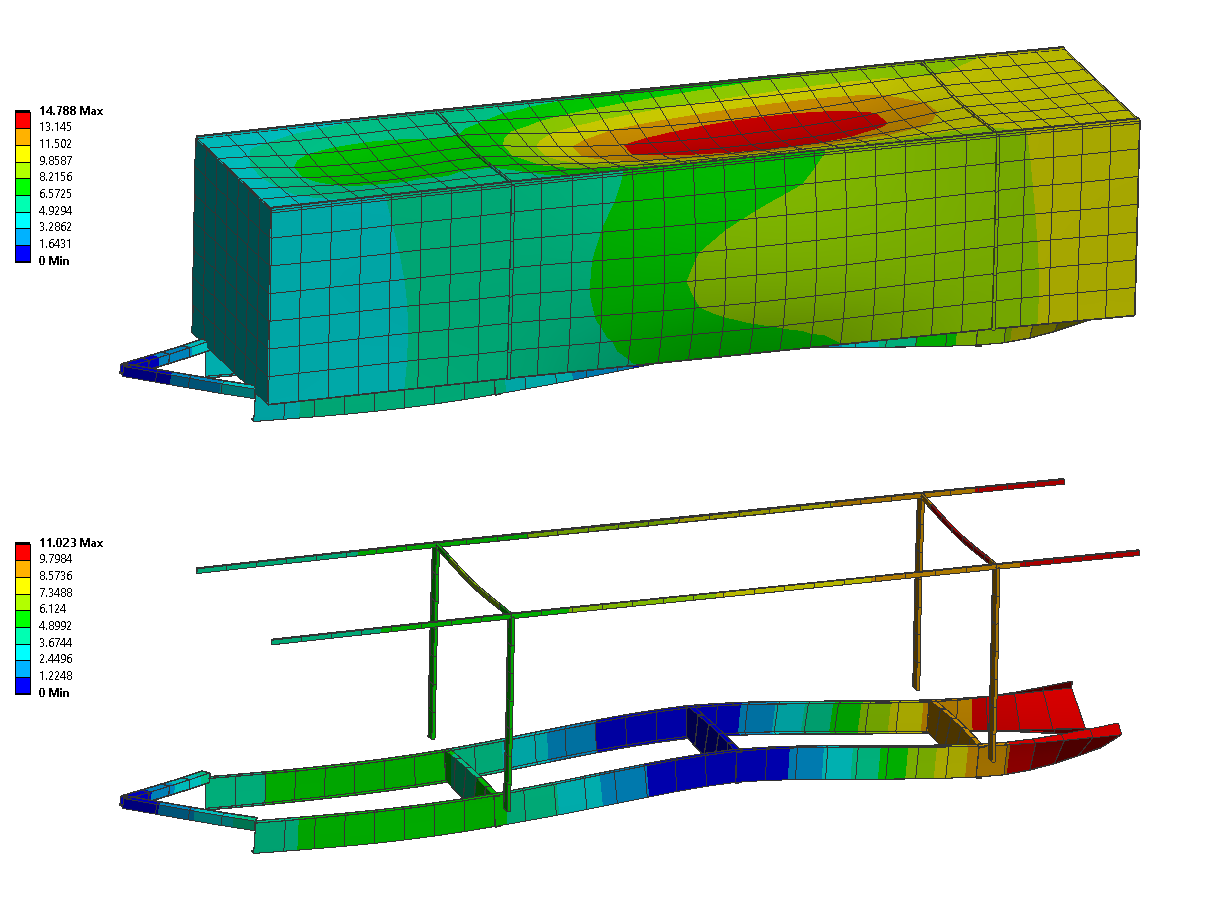
\includegraphics[width=1\linewidth]{04_figures/FEM 1.1.png}
  \caption{Deformation des Solar Butterflys im Lastfall der vertikalen Beschleunigung}
  \label{FEM 1.1}
\end{figure}

\subsubsection{Deformation - Lastfall 1.3 Longitudinale Beschleunigung}
\begin{figure}[H]
  \centering
  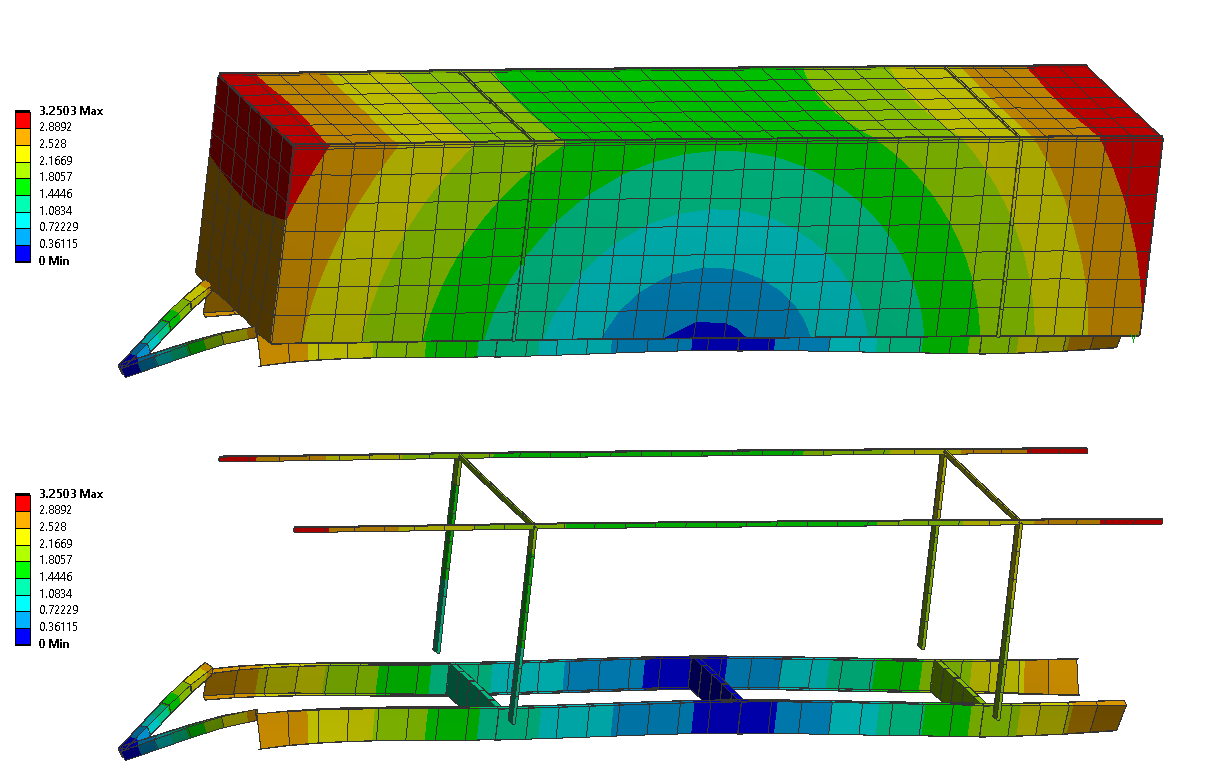
\includegraphics[width=1\linewidth]{04_figures/FEM 1.2.png}
  \caption{Deformation des Solar Butterflys im Lastfall der lateralen Beschleunigung}
  \label{FEM 1.3}
\end{figure}

\subsubsection{Deformation - Lastfall 1.4 Laterale Beschleunigung}
\begin{figure}[H]
  \centering
  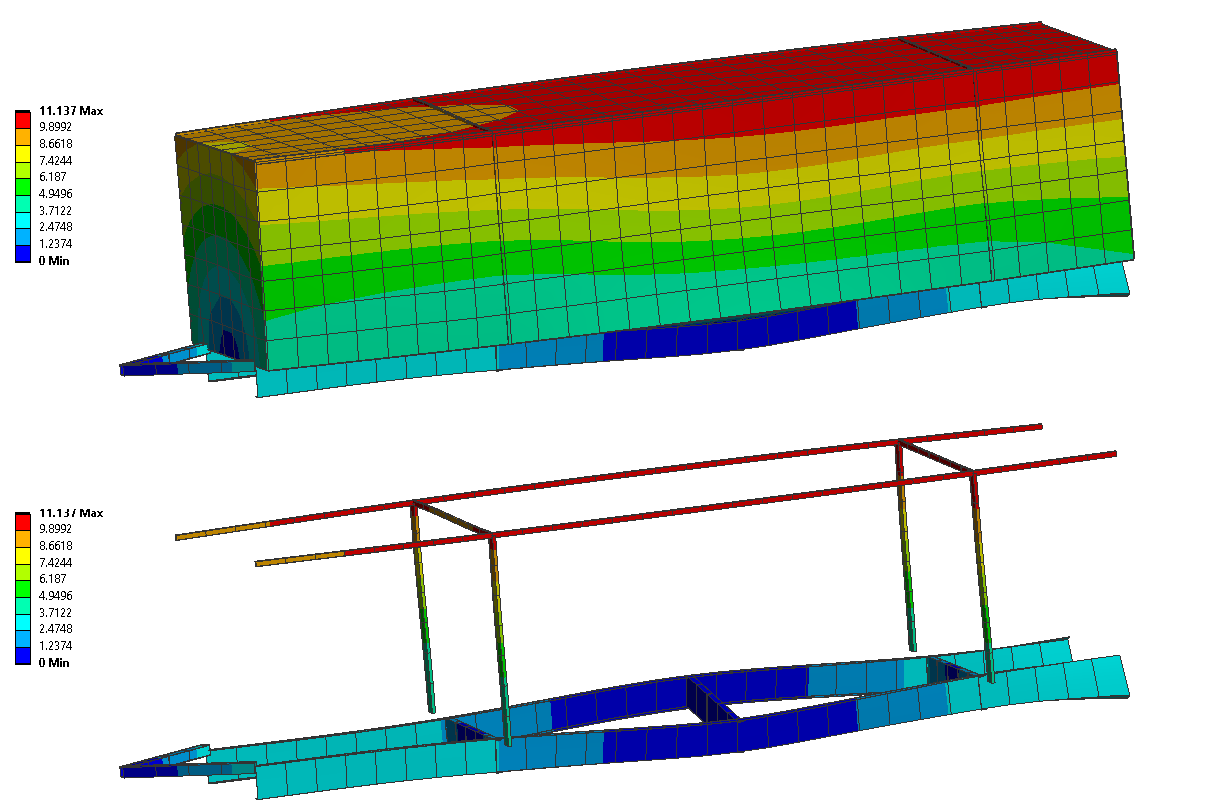
\includegraphics[width=1\linewidth]{04_figures/FEM 1.4.png}
  \caption{Deformation des Solar Butterflys im Lastfall der longitudinalen Beschleunigung}
  \label{FEM 1.4}
\end{figure}

\subsubsection{Deformation - Lastfall 1.5 Rotatorische Beschleunigung}
\begin{figure}[H]
  \centering
  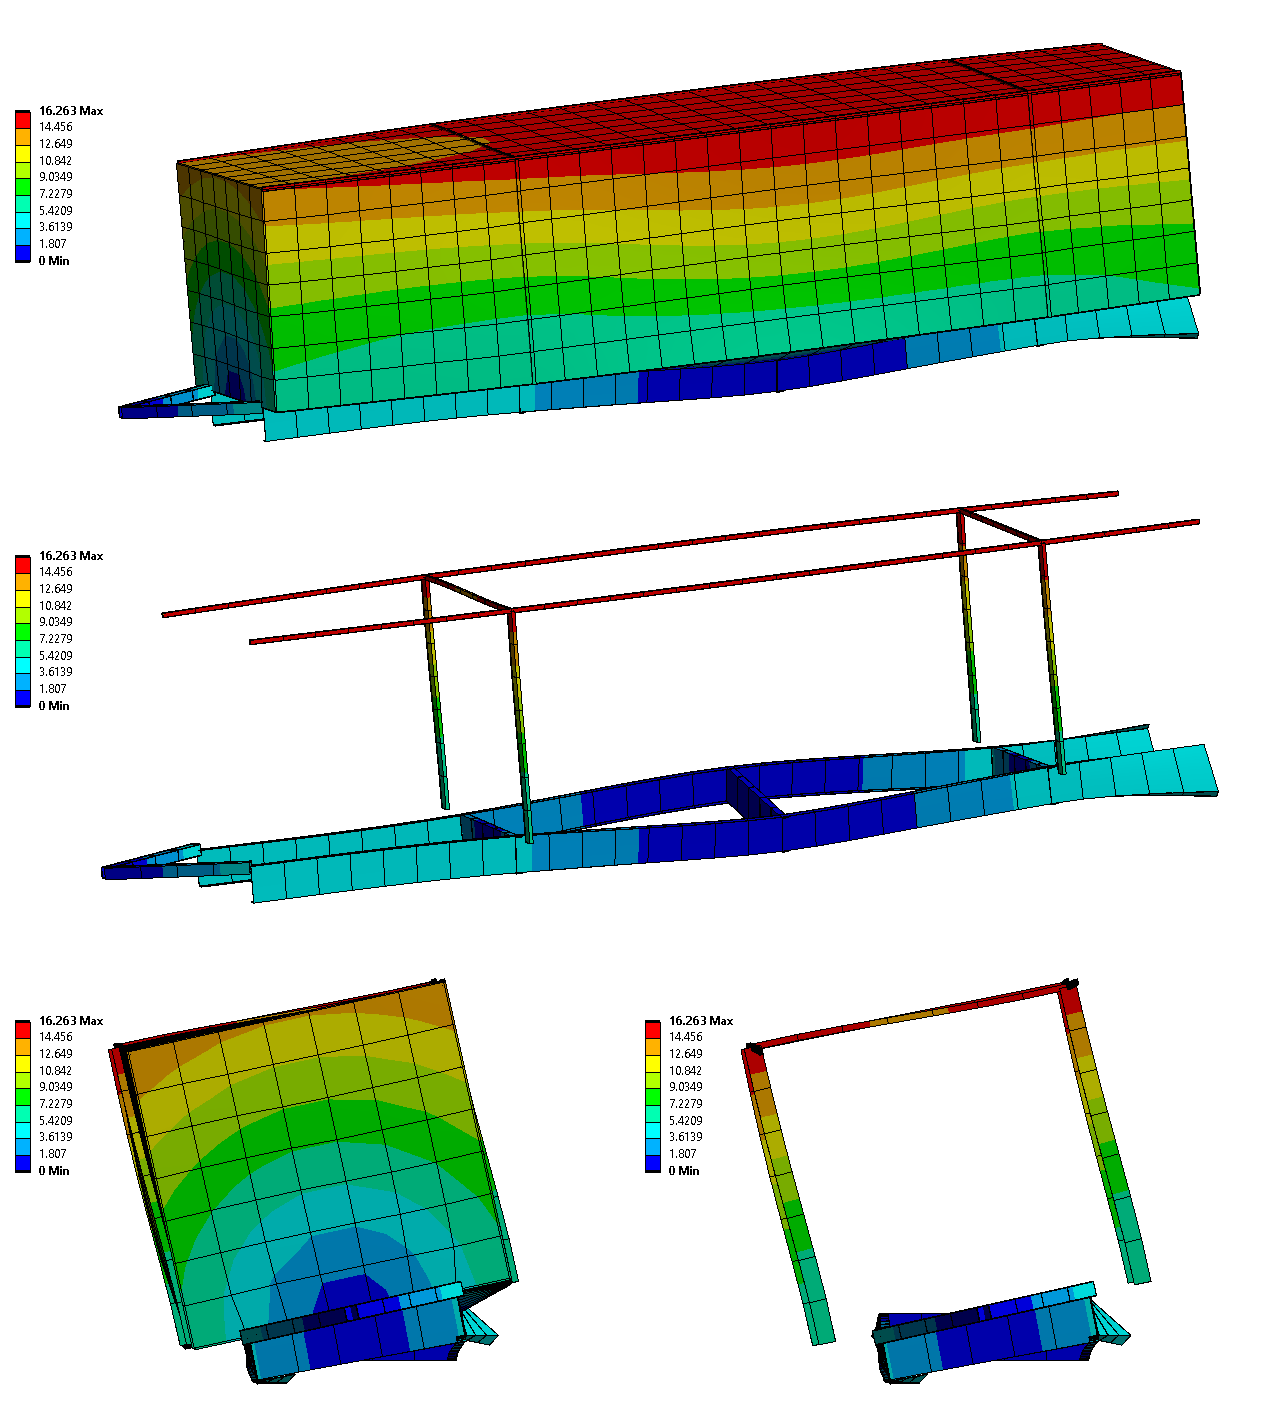
\includegraphics[width=1\linewidth]{04_figures/FEM 1.5.png}
  \caption{Deformation des Solar Butterflys im Lastfall der rotatorischen Beschleunigung}
  \label{FEM 1.5}
\end{figure}
\newpage
